\section{Additional Results}
\label{app:results}
Figures \ref{fig:dimensions} and \ref{fig:tasks} report the size distributions of the datasets. We measure size differently for different types of datasets: Text datasets are in tokens, and audio/video in hours of content. The lack of standard tokenization or preprocessing schemes for those modalities makes it simplest to report raw dataset size.

Notably, we find quite different size distributions by modality. The distribution of dataset sizes has the thickest right tail for text, followed by speech and then by video. Most video datasets are short in hour terms, with speech datasets tending to be somewhat longer and text datasets having a greater prevalence of both very small and very large datasets relative to the mean size.
% More information-rich modalities, in other words, tend to have smaller datasets.

\begin{figure*}[!htb]
    \centering
    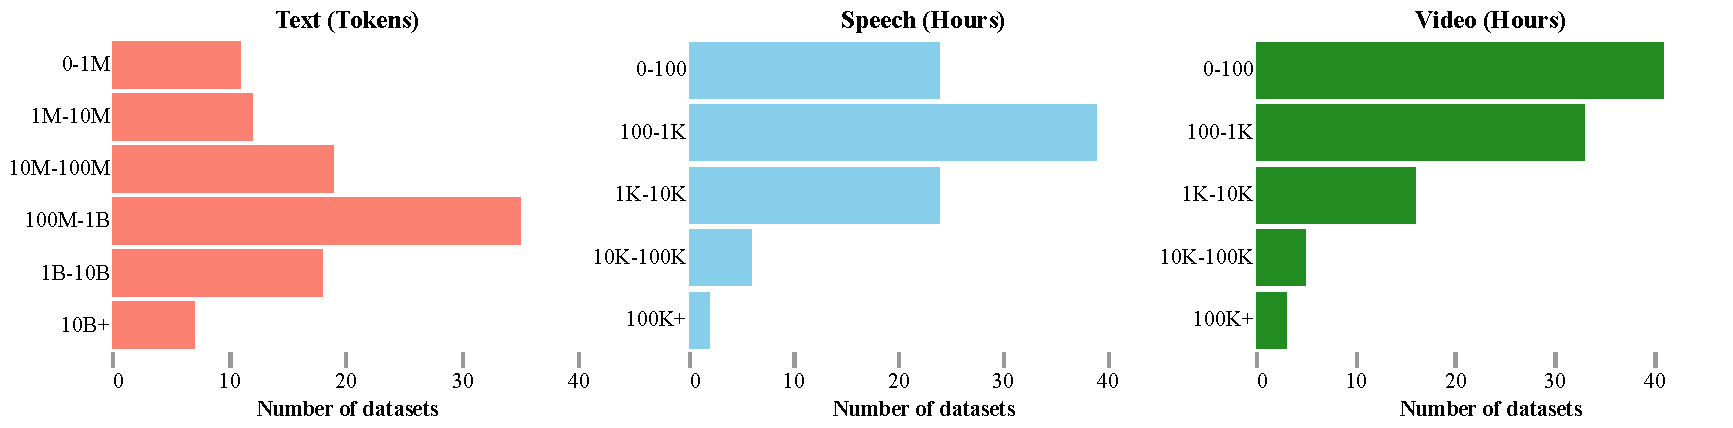
\includegraphics[width=\textwidth]{figures/dimensions.pdf}
    \caption{The distribution of dataset sizes for each modality. Most text data collections are between 100M-1B tokens. \textbf{Speech datasets average 100-1k hours, and video datasets are usually the smallest, commonly less than 100 hours.} }
    \label{fig:dimensions}
\end{figure*}

Dataset tasks, meanwhile, reflect traditional approaches and research programs for each modality. Classification is the most common task for both text and video, with the video community's long-standing interest in captioning also visible in its role as the second most common task for video datasets. Q\&A occupies a similar role for text, though text datasets have a more balanced distribution over other, increasingly prominent tasks like generation and reasoning. Given our selection criteria, all datasets for speech are for ASR tasks, but other tasks like speaker identification and translation are also represented.

\begin{figure*}[!htb]
    \centering
    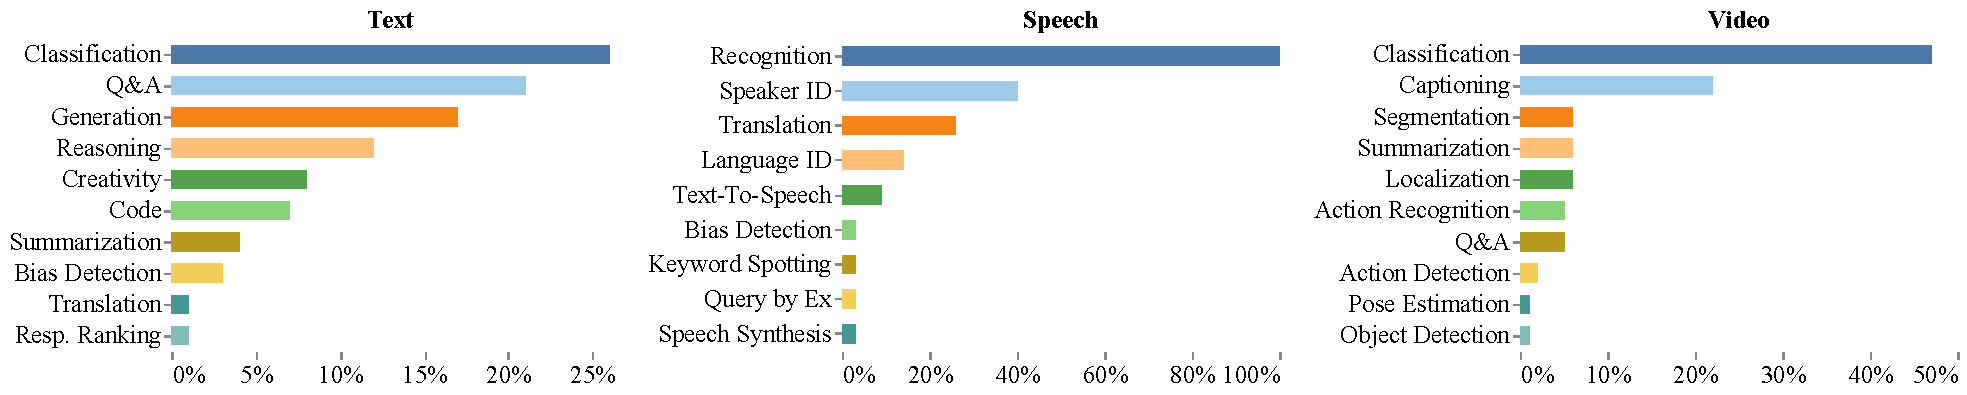
\includegraphics[width=\textwidth]{figures/tasks.pdf}
    \caption{The task distribution of datasets, across modalities. Post-training text and video datasets are predominantly based on classification. For text, generation and reasoning are rising categories. All speech datasets are recognition-based, particularly for speaker, language, or in the process of translation.}
    \label{fig:tasks}
\end{figure*}